\begin{figure}
    \centering
    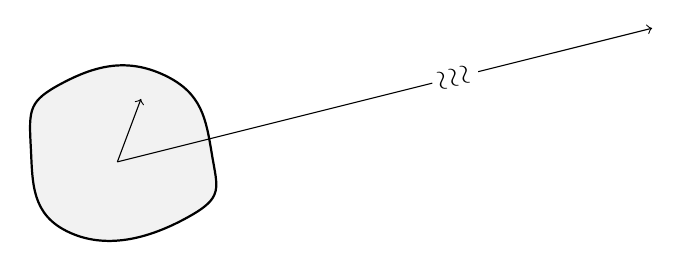
\begin{tikzpicture}
        \def \xa {4}
        \def \ya {1}
        \def \p {0.15}
        \pgfmathsetmacro{\angolo}{atan2(\ya,\xa) + 90}
        \pgfmathsetmacro{\m}{atan2(\ya,\xa)}
        \pgfmathsetmacro{\l}{7}

        \draw[thick, fill=gray!10]
            plot[smooth cycle, tension=0.9] coordinates {
            (1.2,0.1)
            (0.6,1.1)
            (-0.7,1)
            (-1.1,0.2)
            (-0.6,-0.9)
            (0.9,-0.7)
            };

        
        \draw (0,0) -- (\xa,\ya);


        \node[rotate=\angolo] at ({\xa + \p*cos(\m)},{\ya + \p*sin(\m)}) {$\sim$};
        \node[rotate=\angolo] at ({\xa + 2*\p*cos(\m)},{\ya + 2*\p*sin(\m)}) {$\sim$};
        \node[rotate=\angolo] at ({\xa + 3*\p*cos(\m)},{\ya + 3*\p*sin(\m)}) {$\sim$};

        \draw[->] ({\xa + 4*\p*cos(\m)},{\ya + 4*\p*sin(\m)}) -- ({\l*cos(\m)}, {\l*sin(\m)});
        \draw[->] (0,0) -- (0.3,0.8);
        % \draw (0.3,0.8) -- ({\xa}, {\ya + 0.3});
        % \draw[->] ({\xa + 4*\p*cos(\m)},{\ya + 0.3 + 4*\p*sin(\m)}) -- ({\l*cos(\m)}, {\l*sin(\m)});
    \end{tikzpicture}
    \caption{Sorgenti}
    \label{figure:_irraggiamento}
\end{figure}